% ==============================================================================
% PLANTILLA MAESTRA - UnADM (instrucciones comunes)
% ==============================================================================
% Uso rapido:
% 1) Duplica la plantilla y renombra la copia por semana/actividad.
% 2) Actualiza \documenttitle, \documentsubtitle y \documentsubject.
% 3) Lee la planeacion y NO pegues las instrucciones completas dentro del PDF.
%    Usa la planeacion como lista de cumplimiento y redacta con criterio propio.
% 4) Elabora productos visuales preferentemente en LaTeX/TikZ para mantener
%    nitidez y evidencia editable; si usas herramientas externas, inserta
%    capturas de alta resolucion y conserva evidencia dentro del PDF.
% 5) Entrega en PDF con la nomenclatura solicitada en el aula.
%
% Formato institucional (recomendado):
% - Fuente: Helvetica / sans-serif equivalente (\usepackage{helvet}).
% - Interlineado: 1.5 (\onehalfspacing).
% - Citas: autor-año mediante natbib (\citep, \citet, \citep[e.g.][]{clave}).
% - Bibliografía: archivo .bib con formato APA 7; todas las citas del texto
%   deben aparecer en la bibliografía y viceversa.
% - Estructura mínima: portada, resumen/abstract, desarrollo, conclusión y
%   bibliografía.
%
% Reglas para productos visuales y tablas extensas:
% - Para tablas o cuadros amplios use longtable + booktabs y evite líneas
%   verticales; controlar espaciado con \setlength{\tabcolsep} y
%   \renewcommand{\arraystretch}.
% - Para tablas en página propia: use \clearpage, \pagestyle{empty},
%   entorno landscape, reducir tamaño con \scriptsize y luego restaurar
%   \pagestyle{fancy} al finalizar la tabla.
%
% Buenas prácticas de redacción académica (guía operativa):
% - No escribir para llenar espacio; escribir para sostener y defender una idea.
% - Cada concepto debe responder: qué es, qué características tiene, cómo
%   funciona, qué problema resuelve, qué límite presenta y qué implicación
%   jurídica posee.
% - Evitar listas sin análisis: tras cada dato relevante incluya su consecuencia
%   o aplicación jurídica.
% - Primera persona: usar moderadamente ("Considero que", "Desde esta
%   perspectiva"); evite expresiones coloquiales como "yo creo".
%
% Protocolos de integridad y uso de IA:
% - Si se usa IA, el resultado debe ser leído, corregido y transformado con
%   criterio propio. No entregar texto sin procesamiento.
% - Incluir siempre juicio propio y referencias que sostengan la postura.
%
% Checklist operativo antes de entregar:
% [ ] El producto coincide con la técnica solicitada en la planeación.
% [ ] El objetivo y el contenido están alineados con la planeación.
% [ ] El producto visual está rotulado y presentado como se pide.
% [ ] Hay citas APA autor-año dentro del texto y bibliografía completa.
% [ ] No se incluyeron instrucciones copiadas de la planeación dentro del
%     contenido entregado.
% [ ] Ortografía y redacción revisadas; la argumentación es propia.
% ==============================================================================

% CREACION DEL DOCUMENTO
\documentclass[
	spanish,
	letterpaper, oneside
]{article}

% ==============================================================================
% INFORMACION DEL DOCUMENTO
% Actualizar en cada actividad.
% Ejemplos:
% \def\documenttitle {Cuadro comparativo de escuelas clasicas de la etica}
% \def\documentsubtitle {Actividad 2 - Etica y Moral juridica}
% \def\documentsubject {Actividad Semana 2}
% ==============================================================================
\def\documenttitle {Título de la actividad}
\def\documentsubtitle {Actividad X - Ética y Moral jurídica}
\def\documentsubject {Actividad Semana X}

\def\documentauthor {Martín Jonathan de la Cruz}
\def\coursename {Ética y Moral jurídica}
\def\coursecode {030}

\def\universityname {Universidad Abierta y a Distancia de México}
\def\universityfaculty {Licenciatura en Derecho}
\def\universitydepartment {Ética y Moral jurídica}
\def\universitydepartmentimage {departamentos/UnADM}
\def\universitydepartmentimagecfg {height=1.57cm}
\def\universitylocation {Roma Norte, Ciudad de México}

% INTEGRANTES, PROFESORES Y FECHAS
\def\authortable {
	\begin{tabular}{ll}
		\textbf{Alumno:}
		& \begin{tabular}[t]{l}
			 Martín Jonathan de la Cruz \\
		\end{tabular} \\
		Matrícula: & ES2611202040 \\

		\textit{Profesor:}
		& \begin{tabular}[t]{l}
			Emma Liliana \\ Padilla Cano
		\end{tabular} \\
		& \\
		\multicolumn{2}{l}{Fecha de realización: \today} \\
		\multicolumn{2}{l}{\universitylocation}
	\end{tabular}
}

% IMPORTACION DEL TEMPLATE
\input{template}

% FORMATO SOLICITADO / USADO EN ACTIVIDADES CORREGIDAS
\usepackage{helvet}
\renewcommand{\familydefault}{\sfdefault}

% PRODUCTOS VISUALES EN TIKZ
\usepackage{tikz}
\usetikzlibrary{
	arrows.meta,
	positioning,
	calc,
	matrix,
	fit,
	shapes.geometric,
	shadows.blur
}

% CITAS EN FORMATO AUTOR-ANIO, COMPATIBLE CON APA 7 EN EL CUERPO DEL TEXTO
% Usar:
% - Cita parentetica: \citep{clave}
% - Cita narrativa: \citet{clave}
% - Varias fuentes: \citep{clave1,clave2}
\setcitestyle{authoryear,open={(},close={)}}

% ==============================================================================
% AYUDAS DE REDACCION
% Quitar o comentar \pendiente cuando el documento final este terminado.
% ==============================================================================
\newcommand{\pendiente}[1]{\textcolor{red}{[PENDIENTE: #1]}}

\begin{document}

% PORTADA
\templatePortrait

% CONFIGURACION DE PAGINA Y ENCABEZADOS
\templatePagecfg
\onehalfspacing

% ==============================================================================
% RESUMEN / ABSTRACT
% Debe ser breve, no copiar instrucciones.
% Formula recomendada:
% Tema + objetivo + tecnica/producto + enfoque personal.
% ==============================================================================
\begin{abstractd}
	\textbf{Objetivo:} \pendiente{Redactar el objetivo con verbo academico: analizar, comparar, explicar, evaluar, interpretar o relacionar. Debe coincidir con la planeacion semanal.}

	\textbf{Producto elaborado:} \pendiente{Indicar si es cuadro comparativo, esquema, linea de tiempo, mapa conceptual, resumen, reporte de lectura, analisis de hechos o ensayo.}

	\textbf{Enfoque de analisis:} \pendiente{Enunciar la postura central: que criterio etico/moral se analizara y por que importa para la practica juridica.}
\end{abstractd}

% TABLA DE CONTENIDOS - INDICE
\templateIndex

% CONFIGURACIONES FINALES
\templateFinalcfg

% ======================= INICIO DEL DOCUMENTO =======================

% ==============================================================================
% SECCION 1: INTRODUCCION
% Apertura recomendada:
% - Iniciar con una afirmacion fuerte.
% - Traducir la consigna a problema etico-juridico.
% - Mostrar por que el tema importa para la formacion juridica.
% - Cerrar anticipando el enfoque personal.
%
% Evitar:
% - "En este trabajo hablare de..."
% - "La etica es muy importante..."
% - Definiciones de diccionario sin interpretacion.
% ==============================================================================
\section{Introducción}

\pendiente{Abrir con una afirmacion directa. Ejemplo: "La etica juridica no opera como adorno moral del Derecho; funciona como criterio de control frente al poder, la decision y la responsabilidad profesional."}

\pendiente{Explicar el problema de la actividad: que conceptos, escuelas, hechos, valores o dilemas deben analizarse.}

\pendiente{Cerrar con postura inicial. Ejemplo: "La posicion que guia este trabajo es que el valor de una teoria etica se mide por su capacidad para orientar decisiones juridicas concretas sin perder de vista dignidad, responsabilidad y justicia."}

% ==============================================================================
% SECCION 2: DESARROLLO / ANALISIS
% Organizar segun el producto solicitado:
% - Cuadro comparativo: escuela/concepto, definicion, caracteristicas,
%   fundamento, pregunta clave, critica, autor y aplicacion juridica.
% - Esquema: concepto central, ramas principales, notas de funcion y limites.
% - Linea de tiempo: periodo, autor, escuela, aporte, consecuencia etica/juridica.
% - Mapa conceptual: conceptos unidos por conectores verbales claros.
% - Resumen: tesis central de la lectura, argumentos, conceptos y cierre personal.
% - Reporte de lectura: ficha, objetivo, ideas centrales, analisis y valoracion.
% - Analisis de hechos: hechos, problema etico, criterios, valoracion, postura.
% - Ensayo: tesis, argumentos, contraargumento, postura y conclusion.
%
% Regla de parrafo:
% Entrada: concepto o problema.
% Proceso: explicacion, fuente y relacion.
% Salida: consecuencia etica, moral o juridica.
% ==============================================================================
\section{Desarrollo}

\subsection{Contexto y problema}

\pendiente{Presentar el contexto del tema en Etica y Moral juridica. Relacionar con conducta humana, moral social, dignidad, derechos, deber profesional o decision juridica.}

\pendiente{Transformar la consigna en problema operativo: que hay que comparar, organizar, resumir, explicar o valorar.}

\subsection{Análisis conceptual}

\pendiente{Explicar conceptos centrales con fuentes. Cada definicion debe incluir caracteristicas y funcion. Ejemplo de cita APA: \citep{ronquilloarmasEticaGeneralProfesional2018}.}

\pendiente{No acumular autores como lista. Comparar por criterio: bien, deber, placer, virtud, dignidad, responsabilidad, consecuencia, contexto o justicia.}

\subsection{Aplicación jurídica}

\pendiente{Aterrizar el tema a un dilema juridico, derechos humanos, dignidad humana, responsabilidad profesional, CNDH, funcion judicial, legislacion, victimas o justicia social.}

\pendiente{Incluir lectura personal academica: que criterio parece mas util, que limite se observa y que riesgo aparece si se aplica de forma automatica.}

% ==============================================================================
% BLOQUE OPCIONAL: CUADRO COMPARATIVO
% Usar cuando la actividad pida cuadro comparativo.
% Rubrica de referencia:
% - Conceptos precisos.
% - Caracteristicas claras.
% - Redaccion y ortografia.
% - APA 7 en citas y referencias.
% ==============================================================================
%
% \clearpage
% \pagestyle{empty}
% \begin{landscape}
% \begingroup
% \scriptsize
% \setlength{\tabcolsep}{4pt}
% \renewcommand{\arraystretch}{1.35}
% \begin{longtable}{@{}p{0.16\linewidth}p{0.13\linewidth}p{0.13\linewidth}p{0.13\linewidth}p{0.13\linewidth}p{0.13\linewidth}p{0.13\linewidth}@{}}
% \caption{Cuadro comparativo de escuelas eticas}\label{tab:cuadro-etico}\\
% \toprule
% \textbf{Criterio} &
% \textbf{Escuela 1} &
% \textbf{Escuela 2} &
% \textbf{Escuela 3} &
% \textbf{Escuela 4} &
% \textbf{Escuela 5} &
% \textbf{Escuela 6} \\
% \midrule
% \endfirsthead
% \toprule
% \textbf{Criterio} & \textbf{Escuela 1} & \textbf{Escuela 2} & \textbf{Escuela 3} & \textbf{Escuela 4} & \textbf{Escuela 5} & \textbf{Escuela 6} \\
% \midrule
% \endhead
% \midrule
% \multicolumn{7}{r}{Continua en la siguiente pagina} \\
% \endfoot
% \bottomrule
% \endlastfoot
%
% Concepto &
% [Definicion precisa.] &
% [Definicion precisa.] &
% [Definicion precisa.] &
% [Definicion precisa.] &
% [Definicion precisa.] &
% [Definicion precisa.] \\
% \midrule
%
% Caracteristicas &
% [3 rasgos claros.] &
% [3 rasgos claros.] &
% [3 rasgos claros.] &
% [3 rasgos claros.] &
% [3 rasgos claros.] &
% [3 rasgos claros.] \\
% \midrule
%
% Pregunta etica &
% [Pregunta que guia la escuela.] &
% [Pregunta que guia la escuela.] &
% [Pregunta que guia la escuela.] &
% [Pregunta que guia la escuela.] &
% [Pregunta que guia la escuela.] &
% [Pregunta que guia la escuela.] \\
% \midrule
%
% Critica o limite &
% [Riesgo filosofico o juridico.] &
% [Riesgo filosofico o juridico.] &
% [Riesgo filosofico o juridico.] &
% [Riesgo filosofico o juridico.] &
% [Riesgo filosofico o juridico.] &
% [Riesgo filosofico o juridico.] \\
%
% \end{longtable}
% \endgroup
% \end{landscape}
% \pagestyle{fancy}

% ==============================================================================
% BLOQUE OPCIONAL: ESQUEMA EN TIKZ
% Usar cuando la actividad pida esquema. Mantener jerarquia clara:
% titulo -> conceptos principales -> ideas secundarias -> criticas/aplicacion.
% ==============================================================================
%
% \clearpage
% \begin{figure}[H]
% \centering
% \resizebox{0.95\linewidth}{!}{%
% \begin{tikzpicture}[
% 	root/.style={rectangle, rounded corners=2pt, draw=black, fill=black!10,
% 		text width=4cm, align=center, minimum height=1.2cm, font=\bfseries},
% 	nodebox/.style={rectangle, rounded corners=2pt, draw=black!60, fill=gray!8,
% 		text width=4cm, align=center, minimum height=1cm, font=\small},
% 	edge/.style={-{Stealth[length=2.2mm]}, thick, black!55}
% ]
% \node[root] (centro) {Tema central};
% \node[nodebox, below left=1.3cm and 3cm of centro] (a) {Idea principal 1};
% \node[nodebox, below=1.3cm of centro] (b) {Idea principal 2};
% \node[nodebox, below right=1.3cm and 3cm of centro] (c) {Idea principal 3};
% \draw[edge] (centro) -- (a);
% \draw[edge] (centro) -- (b);
% \draw[edge] (centro) -- (c);
% \end{tikzpicture}}
% \caption{Esquema de [tema]}
% \label{fig:esquema}
% \end{figure}

% ==============================================================================
% BLOQUE OPCIONAL: LINEA DE TIEMPO EN TIKZ
% Usar cuando la actividad pida linea de tiempo.
% Cada punto debe tener fecha, autor/escuela, aporte y consecuencia.
% ==============================================================================
%
% \clearpage
% \begin{figure}[H]
% \centering
% \begin{tikzpicture}[
% 	event/.style={rectangle, rounded corners=2pt, draw=black!60, fill=gray!8,
% 		text width=3.4cm, align=center, font=\scriptsize, inner sep=5pt},
% 	dot/.style={circle, fill=black, inner sep=2pt}
% ]
% \draw[thick, -{Stealth[length=2.5mm]}] (0,0) -- (14,0);
% \foreach \x/\year/\text in {
% 	0.8/{Año}/{Aporte principal},
% 	4.0/{Año}/{Aporte principal},
% 	7.2/{Año}/{Aporte principal},
% 	10.4/{Año}/{Aporte principal},
% 	13.0/{Año}/{Aporte principal}
% }{
% 	\node[dot] at (\x,0) {};
% 	\node[event, above=0.45cm of {( \x,0 )}] {\textbf{\year}\\\text};
% }
% \end{tikzpicture}
% \caption{Linea de tiempo de [tema]}
% \label{fig:linea-tiempo}
% \end{figure}

% ==============================================================================
% SECCION 3: POSTURA / ANALISIS PERSONAL
% Esta seccion ayuda a que el producto no se perciba como simple reproduccion.
% Debe contestar:
% - Que posicion se sostiene.
% - Por que esa posicion es razonable.
% - Que fuente o argumento la respalda.
% - Como se aplica a la practica juridica.
% ==============================================================================
\section{Postura personal}

\pendiente{Redactar una posicion clara. Ejemplo: "La posicion que sostengo es que una decision juridica eticamente defendible no depende solo de cumplir una norma, sino de reconocer sus efectos sobre la dignidad y la responsabilidad social."}

\pendiente{Justificar con causa-efecto-consecuencia: si una escuela etica privilegia cierto criterio, entonces produce cierto tipo de decision; por eso conviene usarla con limites.}

\pendiente{Aterrizar a la formacion como abogado: que permite decidir, interpretar, argumentar, cuestionar o proteger.}

% ==============================================================================
% SECCION 4: CONCLUSION
% Debe cerrar con fuerza:
% - Sintetizar el hallazgo.
% - Reafirmar postura.
% - Indicar aplicacion real.
% - Evitar repetir la introduccion.
% ==============================================================================
\section{Conclusión}

\pendiente{Sintetizar el resultado: que se comprendio, que relacion se encontro entre etica, moral y Derecho, y que criterio queda como mas relevante para la actividad.}

\pendiente{Reafirmar postura personal con aplicacion: "Para la practica juridica, este enfoque resulta relevante porque..."}

\pendiente{Cerrar con una frase de consecuencia: que cambia en la forma de interpretar, argumentar o aplicar el Derecho.}

% ==============================================================================
% MANUAL OPERATIVO DE TECNICAS DIDACTICAS
% Este archivo funciona como memoria para futuras sesiones y como guia de
% elaboracion. Para una entrega final, comentar la siguiente linea si el manual no
% debe aparecer dentro del PDF de la actividad.
% ==============================================================================
% ==============================================================================
% MANUAL OPERATIVO: TECNICAS DIDACTICAS DEL APRENDIZAJE
% Fuente de referencia: Coleccion "100 Tecnicas Didacticas de Ensenanza y
% Aprendizaje", Fasciculos 1 a 5, UnADM, 2023.
%
% Proposito del archivo:
% - Servir como guia para elegir, construir y revisar productos didacticos.
% - Traducir la tecnica solicitada en un producto LaTeX/TikZ verificable.
% - Evitar entregas genericas: todo producto debe tener estructura, criterio,
%   analisis y postura cuando la actividad lo permita.
%
% Regla general para nuevas actividades:
% Si la planeacion pide tabla, cuadro comparativo, mapa conceptual, mapa mental,
% linea de tiempo, diagrama, esquema, matriz, cronologia, red conceptual,
% histograma, flujo o proceso, construirlo preferentemente con TikZ/LaTeX.
% Usar captura externa solo si la consigna exige una herramienta especifica o si
% el producto requiere una plataforma interactiva.
% ==============================================================================

\clearpage
\section{Manual operativo de técnicas didácticas}

\subsection{Regla base para productos visuales}

Cuando la actividad solicite un producto visual, el producto debe construirse como parte del documento y no como un elemento improvisado. La regla de trabajo es: si el producto puede representarse con nodos, flechas, tablas, matrices, líneas, ciclos, mapas o relaciones, debe elaborarse en TikZ o con entornos LaTeX como \texttt{tabular}, \texttt{longtable} o \texttt{figure}. Esto permite controlar formato, legibilidad, jerarquía, citas, continuidad visual y coherencia con el documento.

El producto no debe funcionar como adorno. Debe demostrar comprensión: seleccionar información, jerarquizarla, relacionarla y cerrar con una lectura propia. En términos prácticos, cada producto debe contestar cuatro preguntas: qué organiza, con qué criterios lo organiza, qué relación muestra y qué conclusión permite sostener.

\subsection{Estructura común de las técnicas UnADM}

Los fascículos de \textit{100 Técnicas Didácticas de Enseñanza y Aprendizaje} trabajan cada técnica con una lógica estable: definición, estructura, utilidad, proceso de construcción, consideraciones y referencias. Para convertir esa lógica en una actividad universitaria, se recomienda usar esta secuencia:

\begin{enumerate}
	\item \textbf{Identificar el producto solicitado.} No es lo mismo comparar, explicar, analizar, sintetizar o construir. El verbo de la consigna define el nivel de profundidad.
	\item \textbf{Determinar los elementos obligatorios.} Toda técnica tiene piezas mínimas: categorías, conceptos, fuentes, etapas, actores, criterios, datos, ejemplos o conclusiones.
	\item \textbf{Elegir el formato TikZ/LaTeX.} Tabla para comparar, nodos para mapas, flechas para procesos, línea horizontal para cronologías, matriz para decisiones.
	\item \textbf{Redactar antes de diseñar.} El diseño no corrige una idea débil. Primero se definen conceptos y relaciones; después se dibuja.
	\item \textbf{Agregar lectura crítica.} El producto debe mostrar qué significa la información, por qué importa y cómo se aplica.
	\item \textbf{Cerrar con postura.} Si la actividad pide conclusión, debe responder de forma directa la pregunta final y justificarla.
\end{enumerate}

\subsection{Taxonomía de ejecución}

La colección clasifica las técnicas por nivel de ejecución. Esta lectura ayuda a decidir qué profundidad debe tener la entrega:

\begin{longtable}{@{}p{0.14\linewidth}p{0.2\linewidth}p{0.56\linewidth}@{}}
\toprule
\textbf{Nivel} & \textbf{Acción} & \textbf{Criterio para la actividad} \\
\midrule
\endhead
1 & Recordar & Recuperar datos, conceptos, nombres o hechos. Requiere precisión, pero no basta para una actividad universitaria completa. \\
2 & Explicar & Aclarar el significado de un concepto y su función. Debe incluir ejemplos o aplicación. \\
3 & Aplicar & Usar el conocimiento en una situación, caso, norma o problema. Debe mostrar procedimiento. \\
4 & Analizar & Separar elementos, identificar causas, efectos, relaciones y límites. Exige postura crítica. \\
5 & Sintetizar & Integrar información dispersa en un producto ordenado. Debe mostrar jerarquía y selección. \\
6 & Construir & Crear un producto, propuesta, estrategia, guion, ensayo, proyecto o solución. Exige diseño completo y justificación. \\
\bottomrule
\end{longtable}

\subsection{Manual por producto frecuente}

\subsubsection*{Cuadro comparativo}

Usar cuando la consigna pida comparar corrientes, autores, normas, escuelas, conceptos, textos, versiones o modelos. Debe contener una tabla con conceptos en columnas y categorías en filas. Las categorías no deben ser genéricas: deben permitir contraste real. Para asignaturas de Derecho se recomiendan categorías como concepto, fundamento, autores, principios, función, aplicación, límites y valoración crítica; para Redacción en contextos virtuales conviene usar claridad, coherencia, cohesión, formalidad, objetividad, adecuación al receptor y efecto comunicativo.

\textbf{Construcción:} investigar, seleccionar información relevante, definir categorías, ordenar por jerarquía, redactar celdas breves pero sustanciales, citar fuentes y cerrar con conclusión personal. En TikZ/LaTeX puede hacerse con \texttt{longtable}; si se requiere diseño más visual, usar nodos en matriz.

\textbf{Revisión:} cada fila debe permitir una comparación inmediata; si una categoría no cambia la comprensión, se elimina o se reemplaza.

\subsubsection*{Cuadro sinóptico}

Sirve para organizar un tema de lo general a lo particular. Debe mostrar niveles: tema central, categorías principales, subcategorías y detalles. Es útil para corrientes filosóficas, clasificación de derechos, teorías de justicia o tipos de normas.

\textbf{Construcción:} definir tema central, extraer categorías, ordenar por dependencia lógica y usar llaves, ramas o cajas. En TikZ se recomienda una estructura de árbol con nodos alineados.

\subsubsection*{Mapa conceptual}

Debe mostrar conceptos y relaciones mediante palabras de enlace. No basta con poner cajas conectadas; cada flecha debe decir qué relación existe: causa, implica, deriva, limita, permite, exige, se opone a, fundamenta.

\textbf{Construcción:} seleccionar concepto central, jerarquizar conceptos principales y secundarios, escribir conectores precisos, evitar saturación visual y cerrar con explicación breve del mapa. En TikZ usar nodos jerárquicos con flechas etiquetadas.

\subsubsection*{Mapa mental}

Funciona para explorar asociaciones desde una idea central. A diferencia del mapa conceptual, admite ramas más libres, colores, imágenes o palabras clave. Es útil para lluvia de ideas, conceptos iniciales o planeación de investigación.

\textbf{Construcción:} ubicar idea central, crear ramas principales, agregar subramas, usar palabras breves y cerrar con una interpretación. En TikZ usar nodos radiales o coordenadas polares.

\subsubsection*{Línea de tiempo y cronología ilustrada}

La línea de tiempo organiza eventos por secuencia temporal; la cronología ilustrada agrega apoyo visual o iconográfico. Sirve para evolución del pensamiento jurídico, historia de derechos, reformas constitucionales o desarrollo de una corriente.

\textbf{Construcción:} seleccionar fechas relevantes, ordenar cronológicamente, resumir cada evento, señalar causa o consecuencia y cerrar con lectura histórica. En TikZ usar una línea horizontal con hitos alternados arriba/abajo.

\subsubsection*{Esquema}

El esquema resume una estructura lógica. Puede ser jerárquico, secuencial, causal o temático. Sirve cuando la actividad pide explicar un tema sin llegar a mapa conceptual.

\textbf{Construcción:} identificar tema, dividirlo en partes, ordenar relaciones y redactar con frases breves. En TikZ usar cajas alineadas o árbol simple.

\subsubsection*{Diagrama de flujo}

Representa pasos, decisiones y resultados. Es útil para procedimientos jurídicos, interpretación normativa, juicio de amparo, análisis de caso o toma de decisiones.

\textbf{Construcción:} definir inicio, pasos, decisiones, salidas y cierre. Usar rombos para decisiones, rectángulos para acciones y flechas para secuencia. En TikZ usar \texttt{shapes.geometric} y flechas \texttt{Stealth}.

\subsubsection*{Diagrama de Venn}

Muestra coincidencias y diferencias entre conjuntos. Funciona para comparar derecho/moral, legalidad/justicia, reglas/principios o corrientes filosóficas.

\textbf{Construcción:} definir conjuntos, colocar rasgos exclusivos y zona de intersección. En TikZ usar círculos semitransparentes.

\subsubsection*{Diagrama de Gowin}

Relaciona pregunta central, conceptos, principios, registros, transformaciones y conclusiones. Es útil para analizar un problema de investigación o una norma desde teoría y evidencia.

\textbf{Construcción:} formular pregunta, colocar teoría de un lado y evidencia del otro, derivar conclusión. En TikZ se puede construir con una V central y bloques laterales.

\subsubsection*{Mapa de cajas, mapa semántico y redes conceptuales}

Estos productos organizan conceptos por agrupaciones, campos de significado o conexiones. Son útiles para conceptos jurídicos fundamentales o familias de teorías.

\textbf{Construcción:} agrupar por criterio, no por ocurrencia. Cada caja o nodo debe tener función. En TikZ usar cajas por bloque, colores moderados y flechas solo cuando exista relación real.

\subsubsection*{Mapeo de procesos}

Sirve para describir un sistema operativo: entradas, actividades, responsables, controles y salidas. En Derecho puede aplicarse a etapas de interpretación, aplicación normativa o solución de controversias.

\textbf{Construcción:} definir entrada, proceso, control, salida y retroalimentación. En TikZ usar flujo horizontal o carriles.

\subsubsection*{Gráfico estadístico e histograma}

Usar cuando existan datos cuantitativos. No inventar cifras. Si no hay datos confiables, no usar gráfico estadístico como decoración.

\textbf{Construcción:} definir variable, fuente, escala, unidades y lectura del dato. En LaTeX puede usarse \texttt{tikzpicture} o \texttt{pgfplots} si se habilita el paquete.

\subsubsection*{SQA}

SQA organiza tres momentos: qué sé, qué quiero saber y qué aprendí. Es útil para iniciar y cerrar una investigación.

\textbf{Construcción:} usar tabla de tres columnas. La última columna debe mostrar aprendizaje nuevo, no repetir la primera.

\subsubsection*{Valoración de decisiones}

Permite comparar alternativas con criterios cualitativos o cuantitativos. Es útil para justificar una postura entre corrientes, métodos interpretativos o soluciones de caso.

\textbf{Construcción:} definir alternativas, establecer criterios, asignar pesos, valorar y justificar la decisión. En LaTeX usar tabla o matriz ponderada.

\subsubsection*{Ensayo, informe, artículo, monografía y reporte de investigación}

Son productos escritos. No requieren TikZ salvo que incorporen figuras. Deben tener estructura: introducción con problema, desarrollo con fuentes y análisis, conclusión con postura, y referencias.

\textbf{Construcción:} planteamiento, marco conceptual, análisis, aplicación, postura y cierre. Evitar texto enciclopédico. La voz debe convertir información en criterio.

\subsubsection*{Reseña, resumen, reporte de lectura, sumillado y exegética}

Son productos de lectura y síntesis. Deben demostrar comprensión del texto fuente, no sustituirlo por paráfrasis superficial.

\textbf{Construcción:} identificar tesis, argumentos, conceptos clave, límite del texto y lectura personal. Citar correctamente.

\subsubsection*{Debate, foro, panel, mesa redonda, controversia y suasoria}

Son productos argumentativos. Requieren postura, contraargumentos y cierre. En Derecho son útiles para defender interpretaciones o criterios.

\textbf{Construcción:} tesis, argumentos, evidencia, objeción, respuesta y conclusión. Si se presenta por escrito, usar subtítulos claros.

\subsubsection*{Estudio de caso, análisis de hechos y noticia falsa}

Estos productos trabajan con hechos. Deben distinguir hecho, interpretación, norma/principio, problema y solución.

\textbf{Construcción:} hechos relevantes, problema central, criterios de análisis, aplicación, postura y consecuencia.

\subsubsection*{Cartel, afiche, anuncio, fotomontaje y videocápsula}

Son productos comunicativos y visuales. Si la entrega es PDF, el cartel o afiche puede construirse con TikZ. Si se requiere video, el documento debe incluir guion, enlace, captura y justificación.

\textbf{Construcción:} objetivo, público, mensaje central, jerarquía visual, fuentes y cierre. No saturar texto.

\subsubsection*{Glosario colaborativo}

Debe incluir término, definición propia, fuente, ejemplo y comentario. No basta copiar definiciones.

\textbf{Construcción:} ordenar alfabéticamente o por familias conceptuales; citar fuentes; agregar aplicación jurídica.

\subsubsection*{Portafolio de evidencias digital}

Integra productos y reflexión sobre el proceso. Debe mostrar trayectoria, no solo acumulación.

\textbf{Construcción:} índice, evidencias, explicación de cada evidencia, aprendizaje, correcciones y conclusión.

\subsubsection*{Simulación, sociodrama, juego de roles, juego de negocios y taller}

Son técnicas de actuación o aplicación. Si se entregan por escrito, deben incluir guion, roles, contexto, desarrollo, resultados y reflexión.

\textbf{Construcción:} problema, roles, reglas, escena o dinámica, decisiones, cierre y aprendizaje.

\subsubsection*{Consulta pública, encuesta, grupos focales y entrevista}

Son técnicas de recolección de información. Requieren objetivo, participantes, instrumento, resultados y análisis.

\textbf{Construcción:} delimitar problema, formular preguntas claras, aplicar, organizar resultados, interpretar y cerrar con hallazgos.

\subsection{Catálogo de las 100 técnicas}

\begin{longtable}{@{}p{0.08\linewidth}p{0.35\linewidth}p{0.16\linewidth}p{0.31\linewidth}@{}}
\toprule
\textbf{No.} & \textbf{Técnica} & \textbf{Nivel} & \textbf{Producto sugerido en LaTeX/TikZ} \\
\midrule
\endhead
1 & Cuadro comparativo & Sintetizar & Longtable o matriz TikZ. \\
2 & Cuadro sinóptico & Sintetizar & Árbol jerárquico TikZ. \\
3 & Cuestionario & Explicar & Tabla de preguntas/respuestas. \\
4 & Debate & Aplicar & Guion argumentativo. \\
5 & Diagrama de Gowin & Aplicar & Diagrama V en TikZ. \\
6 & Ejemplificación & Explicar & Tabla concepto-ejemplo-aplicación. \\
7 & Entrevista & Aplicar & Guion y matriz de hallazgos. \\
8 & Esquema & Sintetizar & Cajas jerárquicas TikZ. \\
9 & Glosario colaborativo & Explicar & Tabla término-definición-fuente. \\
10 & Historieta & Recordar & Viñetas TikZ o guion. \\
11 & Informe & Sintetizar & Documento con secciones. \\
12 & Línea de tiempo & Sintetizar & Timeline TikZ. \\
13 & Mapa conceptual & Sintetizar & Nodos y conectores TikZ. \\
14 & Panel de discusión & Aplicar & Tabla de posturas. \\
15 & Pensamiento de diseño & Recordar & Fases empatizar-definir-idear-prototipar-evaluar. \\
16 & Phillips 66 & Aplicar & Matriz grupo-idea-síntesis. \\
17 & Resumen & Recordar & Texto breve estructurado. \\
18 & Simulación & Construir & Escenario, variables y resultados. \\
19 & Sociodrama & Aplicar & Guion de escenas. \\
20 & Trabajo cooperativo & Aplicar & Plan de roles y evidencias. \\
21 & Análisis de contenido & Analizar & Matriz texto-idea-función-crítica. \\
22 & Análisis de tergiversación textual & Analizar & Tabla afirmación/evidencia/corrección. \\
23 & Análisis y consensos & Analizar & Matriz de acuerdos y disensos. \\
24 & Autoexplicación & Explicar & Secuencia pregunta-respuesta-criterio. \\
25 & Cronología ilustrada & Construir & Línea de tiempo con iconos. \\
26 & Estructuras textuales & Analizar & Mapa de estructura argumentativa. \\
27 & Estudio de casos & Explicar & Hechos-problema-norma-solución. \\
28 & Exposición oral & Aplicar & Guion o diapositivas. \\
29 & Foro & Aplicar & Entrada, réplica y cierre. \\
30 & Grupos de discusión & Aplicar & Matriz de aportaciones. \\
31 & Grupos focales & Explicar & Guion y síntesis de hallazgos. \\
32 & Mapa de cajas & Sintetizar & Cajas agrupadas TikZ. \\
33 & Mapa mental & Explicar & Nodos radiales TikZ. \\
34 & Monografía & Explicar & Documento de investigación. \\
35 & Preguntas y premios & Recordar & Banco de reactivos. \\
36 & Reporte de lectura general & Explicar & Ficha de lectura ampliada. \\
37 & Reseña & Sintetizar & Valoración crítica breve. \\
38 & Rompecabezas & Construir & Integración por piezas. \\
39 & Sumillado & Sintetizar & Texto con notas marginales. \\
40 & Testimonio & Recordar & Entrevista y relato analizado. \\
41 & Consulta pública & Aplicar & Instrumento y matriz de resultados. \\
42 & Controversia estructurada & Analizar & Tesis, antítesis y síntesis. \\
43 & Debate público & Aplicar & Guion de argumentación. \\
44 & Diagrama de Venn & Analizar & Círculos TikZ. \\
45 & Diario de aprendizaje & Recordar & Bitácora reflexiva. \\
46 & Discusión de gabinete & Analizar & Tabla de roles y decisiones. \\
47 & Documentales & Explicar & Guion audiovisual. \\
48 & Encuesta interactiva & Aplicar & Instrumento y gráfica. \\
49 & Ensayo & Construir & Texto argumentativo. \\
50 & Estudio de noticia falsa & Analizar & Verificación y contraste de fuentes. \\
51 & Exegética & Recordar & Interpretación textual guiada. \\
52 & Fábula & Recordar & Narración con moraleja. \\
53 & Heurística de Bruner & Analizar & Ruta descubrimiento-concepto. \\
54 & Histograma & Analizar & Gráfico de frecuencias. \\
55 & Pensamiento analógico & Aplicar & Analogía y transferencia. \\
56 & Poesía lírica & Construir & Producto creativo con reflexión. \\
57 & Sesión bibliográfica & Analizar & Fichas por fuente. \\
58 & SQA & Recordar & Tabla sé-quiero-aprendí. \\
59 & Suasoria & Aplicar & Discurso persuasivo. \\
60 & Tablón de anuncios & Sintetizar & Muro informativo o tablero. \\
61 & Afiche & Explicar & Cartel breve en TikZ. \\
62 & Análisis de hechos & Analizar & Hechos-causas-consecuencias. \\
63 & Anuncio publicitario & Explicar & Pieza persuasiva. \\
64 & Atributos & Explicar & Tabla de cualidades. \\
65 & Diagrama de flujo & Sintetizar & Flujo TikZ. \\
66 & Diálogos simultáneos & Aplicar & Guion de interacción. \\
67 & Feynman & Explicar & Explicación simple y prueba. \\
68 & Gráfico estadístico & Analizar & Gráfico con fuente. \\
69 & Lluvia de ideas dirigida & Explicar & Mapa radial o lista clasificada. \\
70 & Mapa semántico & Sintetizar & Red de significados TikZ. \\
71 & Mapeo de procesos & Analizar & Proceso entrada-salida. \\
72 & Mesa redonda con interrogador & Aplicar & Matriz de preguntas/posturas. \\
73 & Mnemotecnia & Recordar & Reglas de memoria. \\
74 & Portafolio de evidencias digital & Construir & Índice de evidencias. \\
75 & Redes conceptuales & Sintetizar & Grafo TikZ. \\
76 & Reporte de investigación & Explicar & Documento con método. \\
77 & Simposio & Aplicar & Programa y síntesis. \\
78 & Socioaprendizaje & Aplicar & Comunidad y evidencias. \\
79 & Tuits & Sintetizar & Microargumentos. \\
80 & Valoración de decisiones & Analizar & Matriz ponderada. \\
81 & Artículo & Analizar & Texto con tesis y fuentes. \\
82 & Cartel & Explicar & Cartel TikZ. \\
83 & Demostración silenciosa & Aplicar & Secuencia visual. \\
84 & Descripción de un personaje & Aplicar & Perfil estructurado. \\
85 & Estudio intercalado & Aplicar & Plan de estudio espaciado. \\
86 & Examen práctico & Aplicar & Evidencia de ejecución. \\
87 & Fotomontaje digital & Construir & Composición visual justificada. \\
88 & Instrucción personalizada & Analizar & Ruta de aprendizaje individual. \\
89 & Journal digital & Construir & Bitácora digital. \\
90 & Juego de negocios & Analizar & Simulación estratégica. \\
91 & Juego de roles & Aplicar & Guion de roles. \\
92 & Práctica distribuida & Aplicar & Calendario de práctica. \\
93 & Preguntas dirigidas & Construir & Banco de preguntas guía. \\
94 & Proyectos colaborativos & Construir & Plan de proyecto. \\
95 & Reportaje & Construir & Investigación narrativa. \\
96 & Scamper & Recordar & Matriz sustituir-combinar-adaptar. \\
97 & Social media & Aplicar & Estrategia de publicación. \\
98 & Taller & Aplicar & Secuencia de actividades. \\
99 & Videocápsula & Sintetizar & Guion y storyboard. \\
100 & Visitas guiadas virtuales 360 & Construir & Guion, secuencia y recorrido. \\
\bottomrule
\end{longtable}

\subsection{Plantillas TikZ mínimas}

Estas plantillas se pueden copiar a la actividad concreta y ajustar.

\subsubsection*{Mapa conceptual}

\begin{verbatim}
\begin{figure}[H]
\centering
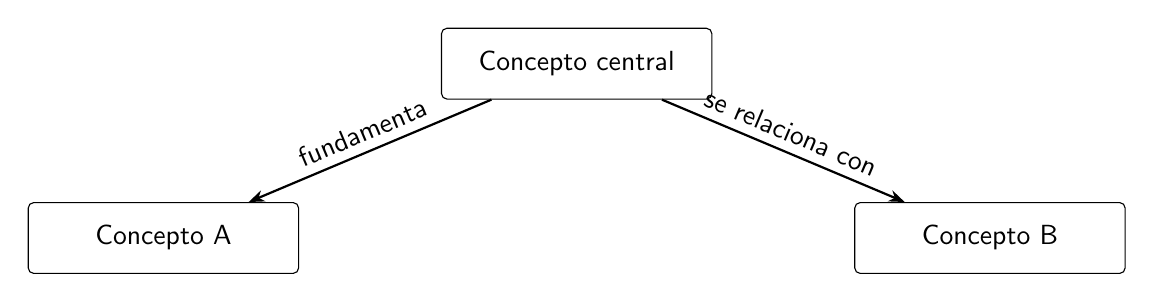
\begin{tikzpicture}[
  concepto/.style={rectangle, draw, rounded corners=2pt,
    align=center, text width=3.2cm, minimum height=0.9cm},
  flecha/.style={-{Stealth[length=2mm]}, thick}
]
\node[concepto] (a) {Concepto central};
\node[concepto, below left=1.3cm and 1.8cm of a] (b) {Concepto A};
\node[concepto, below right=1.3cm and 1.8cm of a] (c) {Concepto B};
\draw[flecha] (a) -- node[above, sloped]{fundamenta} (b);
\draw[flecha] (a) -- node[above, sloped]{se relaciona con} (c);
\end{tikzpicture}
\caption{Mapa conceptual de [tema]}
\end{figure}
\end{verbatim}

\subsubsection*{Línea de tiempo}

\begin{verbatim}
\begin{figure}[H]
\centering
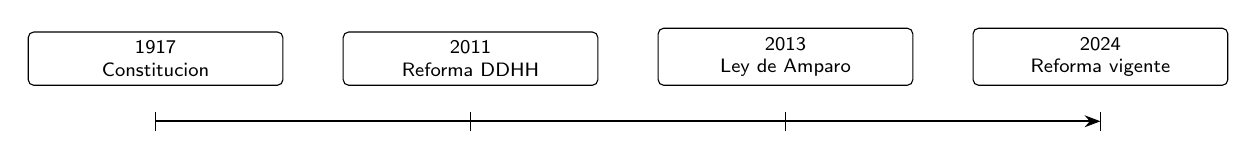
\begin{tikzpicture}[
  evento/.style={rectangle, draw, rounded corners=2pt,
    align=center, text width=3cm, font=\scriptsize},
  eje/.style={-{Stealth[length=2mm]}, thick}
]
\draw[eje] (0,0) -- (12,0);
\foreach \x/\anio/\texto in {
  0/1917/Constitucion,
  4/2011/Reforma DDHH,
  8/2013/Ley de Amparo,
  12/2024/Reforma vigente}
{
  \draw (\x,0.12) -- (\x,-0.12);
  \node[evento, above=0.45cm] at (\x,0) {\anio\\\texto};
}
\end{tikzpicture}
\caption{Linea de tiempo de [tema]}
\end{figure}
\end{verbatim}

\subsubsection*{Diagrama de flujo}

\begin{verbatim}
\begin{figure}[H]
\centering
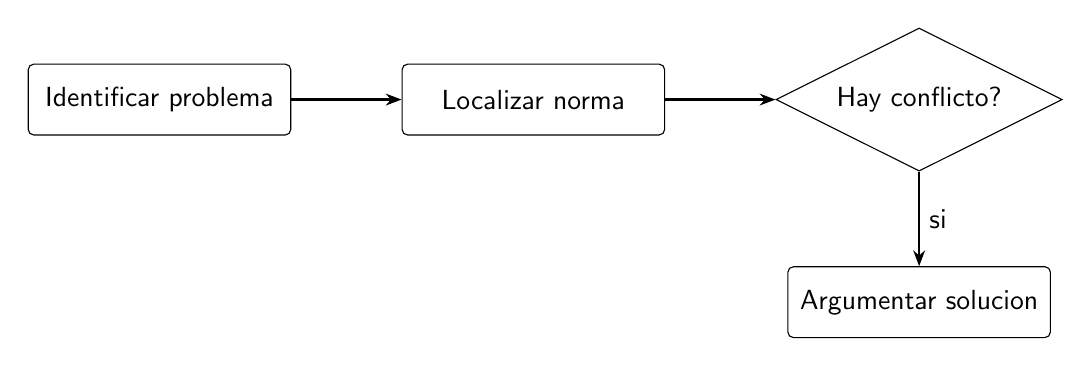
\begin{tikzpicture}[
  paso/.style={rectangle, draw, rounded corners=2pt,
    align=center, text width=3.1cm, minimum height=0.9cm},
  decision/.style={diamond, draw, aspect=2, align=center,
    text width=2.8cm, inner sep=1pt},
  flecha/.style={-{Stealth[length=2mm]}, thick}
]
\node[paso] (inicio) {Identificar problema};
\node[paso, right=1.4cm of inicio] (norma) {Localizar norma};
\node[decision, right=1.4cm of norma] (decision) {Hay conflicto?};
\node[paso, below=1.2cm of decision] (analisis) {Argumentar solucion};
\draw[flecha] (inicio) -- (norma);
\draw[flecha] (norma) -- (decision);
\draw[flecha] (decision) -- node[right]{si} (analisis);
\end{tikzpicture}
\caption{Diagrama de flujo de [proceso]}
\end{figure}
\end{verbatim}

\subsection{Cierre operativo}

La elección de una técnica no debe ser decorativa. Si la actividad pide un producto, la técnica funciona como una herramienta de análisis. El criterio de calidad es que el producto permita ver una decisión intelectual: qué se seleccionó, cómo se organizó, qué relación se construyó y qué postura se puede defender a partir de esa organización.


% ==============================================================================
% REFERENCIAS
% Reglas:
% - Toda fuente citada en el texto debe estar en el .bib.
% - Toda cita debe tener clave correcta.
% - Usar fuentes de la planeacion y, si se complementa, que sean confiables.
% - En el cuerpo: \citep{clave}; no usar solo URLs sueltas.
% ==============================================================================
\bibliography{etica-y-moral-juridica}

% FIN DEL DOCUMENTO
\end{document}


